\documentclass[a4paper,UKenglish,cleveref, autoref, thm-restate,anonymous]{lipics-v2021}

\hideLIPIcs  

\bibliographystyle{plainurl}

\ifx\authoranonymous\relax
\newcommand{\GITHUBURL}{(anonymised)}
\newcommand{\COFFEEURL}{(anonymised)}
\else
\newcommand{\GITHUBURL}{\url{https://github.com/songlarknet/pipit}}
\newcommand{\COFFEEURL}{\url{https://youtu.be/6IybbQFPOl8}}
\fi

\usepackage{mathtools}
\usepackage{mathpartir}

\usepackage{stmaryrd}

\usepackage{wasysym}
\usepackage{underscore}

\usepackage{style/utils}
\usepackage{style/code}
\usepackage{style/proof}
\usepackage{style/keywords}
\usepackage{style/judgements}


\title{Pipit on the Post: Proving Pre- and Post-conditions of Reactive Systems}


\author{Amos Robinson}{Australian National University, Canberra, Australia}{amos.robinson@anu.edu.au}{https://orcid.org/0009-0004-4837-4981}{}

\author{Alex Potanin}{Australian National University, Canberra, Australia}{alex.potanin@anu.edu.au}{https://orcid.org/0000-0002-4242-2725}{}

\authorrunning{A. Robinson and A. Potanin}
\Copyright{Amos Robinson and Alex Potanin}
\ccsdesc[500]{Computer systems organization~Real-time languages}
\ccsdesc[500]{Theory of computation~Program verification}
\ccsdesc[500]{Software and its engineering~Specialized application languages}
\keywords{Lustre, streaming, reactive, verification}



\begin{document}

\maketitle

\begin{abstract}
  Reactive languages such as Lustre and Scade are used to implement safety-critical control systems; proving such programs correct and having the proved properties apply to the compiled code is therefore equally critical.
  We introduce Pipit, a small reactive language embedded in \fstar{}, designed for verifying control systems and executing them in real-time.
  Pipit includes a verified translation to transition systems; by reusing \fstar{}'s existing proof automation, certain safety properties can be automatically proved by k-induction on the transition system.
  Pipit can also generate executable code in a subset of \fstar{} which is suitable for compilation and real-time execution on embedded devices.
  The executable code is deterministic and total and preserves the semantics of the original program.
\end{abstract}


% \makeatactive


\section{Introduction}
Safety-critical control systems, such as the anti-lock braking systems that are present in most cars today, need to be correct and execute in real-time.
One approach, favoured by parts of the aerospace industry, is to implement the controllers in a high-level language such as Lustre~\cite{caspi1995functional} or Scade~\cite{colaco2017scade}, and verify that the implementations satisfy the high-level specification using a model-checker, such as Kind2~\cite{champion2016kind2}.
These model-checkers can prove many interesting safety properties automatically, but do not provide many options for manual proofs when the automated proof techniques fail.
Additionally, the semantics used by the model-checker may not match the semantics of the compiled code, in which case properties proved do not necessarily hold on the real system.
This mismatch may occur even when the compiler has been verified to be correct, as in the case of Vélus~\cite{bourke2017formally}.
For example, in Vélus, integer division rounds towards zero, matching the semantics of C; however, integer division in Kind2 rounds to negative infinity, matching SMT-lib~\cite{BarFT2016SMTLIB,kind2023intdiv}.

To be confident that our proofs hold on the real system, we need a single semantics that is shared between the compiler and the model-checker or prover.
In this paper we introduce Pipit\footnote{Implementation available at \GITHUBURL}, an embedded domain-specific language for implementing and verifying controllers in \fstar{}.
Pipit aims to provide a high-level language based on Lustre, while reusing \fstar{}'s proof automation and manual proofs for verifying controllers~\cite{martinez2019meta}, and using \lowstar{}'s C-code generation for real-time execution~\cite{protzenko2017verified}.
To verify programs, Pipit translates its expression language to a transition system for k-inductive proofs, which is verified to be an abstraction of the original semantics.
To execute programs, Pipit can generate executable code, which is total and semantics-preserving.



In this paper, we make the following contributions:

\begin{itemize}
  \item we motivate the need to combine manual and automated proofs of reactive systems with a strong specification language (\autoref{s:motivation});
  \item we introduce Pipit, a minimal reactive language that supports rely-guarantee contracts and properties; crucially, proof obligations are annotated with a status --- \emph{valid} or \emph{deferred} --- allowing proofs to be delayed until more is known of the program context (\autoref{s:core});
  \item we describe a \emph{checked semantics} for Pipit, which is parameterised by the property status; after checking deferred properties, programs can be \emph{blessed}, and their properties lifted to valid status (\autoref{s:core:checked});
  \item we describe an encoding of transition systems that can express under-specified rely-guarantee contracts as functions rather than relations; composing functions results in simpler transition systems (\autoref{s:transition});
  \item we identify the invariants and lemmas required to prove that the abstract transition system is an abstraction of the original semantics (\autoref{s:core:causality}, \autoref{s:transition:proof});
  \item similarly, we offer a mechanised proof that the executable transition system preserves the original semantics (\autoref{s:extraction});
  \item finally, we evaluate Pipit by implementing the high-level logic of a time-triggered Controller Area Network (CAN) bus driver and verifying an abstract model of a key operation (\autoref{s:evaluation}).
\end{itemize}
 

\section{Pipit for time-triggered networks}
\label{s:motivation}



To introduce Pipit, we consider a driver with a static schedule of \emph{triggers}, or actions to be performed at a particular time; this driver is a simplification of the time-triggered Controller Area Network (CAN) bus specification \cite{fuehrer2001time} which we will discuss further in \autoref{s:evaluation}.


\subsection{Deferring and proving properties}

The schedule of our time-triggered driver is determined by a constant array of triggers, sorted by their associated time-mark.
The driver maintains an index that refers to the current trigger.
At each instant in time, the driver checks if the current trigger has expired or is inactive, and if so, it increments the index.
We first implement a streaming function \emph{count_when} to maintain the index; the function takes a constant natural number \emph{max} and a stream of booleans \emph{inc}.
At each time step, \emph{count_when} checks whether the current increment flag is true; if so, it increments the previous counter, saturating at the maximum; otherwise, it leaves the previous counter as-is.

\begin{tabbing}
  \tt{MM}\= \tt{MM} \= \kill
  \tt{let} count_when ($\textit{max}$: $\NN$) ($\textit{inc}$: stream $\BB$): stream $\NN$ = \\
    \> $\tt{rec}~\rawbind{\textit{count}}{}$ \\
    \> \> $\xcheckP{\PSUnknown}{(0 \le \textit{count} \le \textit{max})}$; \\
    \> \> \tt{let} $\textit{count'}$ \tt{=} $(0~\tt{fby}~\textit{count}) + (\tt{if}~\textit{inc}~\tt{then}~1~\tt{else}~0)$ \tt{in} \\
    \> \> \tt{if } $\textit{count'} \ge \textit{max}$ \tt{then} $\textit{max}$  \tt{else} $\textit{count'}$
\end{tabbing}

The implementation of \emph{count_when} first defines a recursive stream, \emph{count}, which states an invariant about the count before defining the incremented stream \emph{count'}.
Inside \emph{count'}, the syntax $0~\tt{fby}~\textit{count}$ is read as ``the initial value of zero \emph{followed by} the previous count''.

The syntax $\xcheckP{\PSUnknown}{(0 \le \textit{count} \le \textit{max})}$ asserts that the count is within the range $[0, \textit{max}]$.
The subscript $\PSUnknown$ on the check is the \emph{property status}, which in this case denotes that the assertion has been stated, but it is not yet known whether it holds.
A property status of $\PSValid$, on the other hand, denotes that a property has been proved to hold.
These property statuses are used to defer checking properties until enough is known about the environment, and to avoid rechecking properties that have already been proven.
In practice, the user does not explicitly specify property statuses in the source language.
The stated property $(0 \le \textit{count} \le \textit{max})$ is a stream of booleans which must always be true.
Non-streaming operations such as $\le$ are implicitly lifted to streaming operations, and non-streaming values such as $0$ and $\textit{max}$ are implicitly lifted to constant streams.

We defer the proof of the property here because, at the point of stating the property inside the \tt{rec} combinator, we don't yet have a concrete definition for the count variable.
In this case, we could have instead deferred the \emph{statement} of the property by introducing a let-binding for the recursive count and putting the \tt{check} outside of the \tt{rec} combinator.
However, it is not always possible to defer property statements: for example, when calling other streaming functions that have their own preconditions, it may not be possible to move the function call outside of its enclosing \tt{rec}.


Pipit is an embedded domain-specific language.
The program above is really syntactic sugar for an \fstar{} program that takes a natural number and constructs a Pipit core expression with a free boolean variable.
We will discuss the details of the core language in \autoref{s:core}, but for now we focus on the source program with some minor embedding details omitted.

To actually prove the property above, we use the meta-language \fstar{}'s tactics to translate the program into a transition system and prove the property inductively on the system.
Finally, we \emph{bless} the expression, which marks the properties as valid ($[\PSUnknown := \PSValid]$).
Blessing is an intensional operation that traverses the expression and updates the internal metadata, but does not affect the runtime semantics.

\begin{tabbing}
  \tt{MM}\= \tt{MM} \= \kill
  \tt{let} $\mbox{count_when}_{\PSValid}$ ($\textit{max}$: $\NN$): stream $\BB$ $\to$ stream $\NN$ = \\
    \> \tt{let} $\textit{system} = \mbox{System.translate}_1 (\mbox{count_when}~\textit{max})$ \tt{in} \\
    \> \tt{assert} (System.inductive_check $\textit{system}$) \tt{by} (pipit_simplify ()); \\
    \> $\tt{bless}_1$ $(\mbox{count_when}~\textit{max})$
\end{tabbing}

The subscript 1 in the translation to transition system and blessing operations refers to the fact that the stream function has one stream parameter.
The \emph{pipit_simplify} tactic in the assertion performs normalisation-by-evaluation to simplify away the translation to a first-order transition system; \fstar{}'s proof-by-SMT can then solve the inductive check directly.


Callers of \emph{count_when} can now use the validated variant without needing to re-prove the count-range property.
In a dedicated model-checker such as Kind2 \cite{champion2016kind2} or Lesar \cite{raymond2008synchronous}, this kind of bookkeeping would all be performed under-the-hood.
By embedding Pipit in a general-purpose theorem prover, we move some of the bookkeeping burden onto the user; however, we have increased confidence that the compiled code matches the verified code and, as we shall see, we also have access to a rich specification language.


\subsection{The time-triggered system matrix}

The schedule of the time-triggered network is abstractly described by a \emph{system matrix}, consisting of rows of \emph{basic cycles}, columns of \emph{transmission columns}, and cells of optional messages.
Each basic cycle is identified by its cycle index and each transmission column has an associated time-mark.

\autoref{f:tt-systemmatrix-ok} (left) shows an example system matrix with cycles \tt{C0} and \tt{C1} and transmission columns at time-marks 0, 1 and 2.
For this example, we assume that one message can be sent per clock cycle. To execute this system matrix, we synchronise the local time to zero at the start of basic cycle \tt{C0}.
After a basic cycle completes, the nodes on the network synchronise before execution continues to the next basic cycle.

\autoref{f:tt-systemmatrix-ok} (right) shows the corresponding configuration for the triggers array.
The enabled set denotes the basic cycles for which a trigger is active.

The system has strict timing requirements which restrict how triggers can be defined.
In this example, each trigger has a unique time; in general, trigger times can overlap, but they need to be enabled on distinct cycles.
Additionally, the schedule must allow sufficient time for the driver to skip over the disabled triggers.
Concretely, we could postpone trigger 1 to send message \tt{B} at time-mark 2, as triggers 1 and 2 have distinct cycles.
However, we could not bring forward trigger 2 to send message \tt{C} at time-mark 1: the driver can only process one trigger per tick, and it takes two steps to reach trigger 2 from the start of the array.

\begin{figure}
  \begin{minipage}{0.38\textwidth}
\begin{tabular}{r|ccc}
   & TM0 & TM1 & TM2 \\
  \hline
  C0 & MSG A & MSG B & - \\
  C1 & MSG A & - & MSG C
\end{tabular}
\end{minipage}
\begin{minipage}{0.6\textwidth}
\small
\begin{verbatim}
  0: { time_mark = 0; enabled = {C0,C1}; msg = A; }
  1: { time_mark = 1; enabled = {C0};    msg = B; }
  2: { time_mark = 2; enabled = {C1};    msg = C; }
\end{verbatim}
\end{minipage}
  
\caption{Left: system matrix; right: corresponding triggers array configuration}
\label{f:tt-systemmatrix-ok}
\end{figure}



We impose three restrictions on the triggers array: the time-marks must be sorted; there must be an adequate time-gap between any two triggers that are enabled on the same cycle index; and each trigger's time-mark must be greater-than-or-equal to its index.

With these restrictions in place, we prove a lemma \emph{lemma_can_reach_next}, which states that for all valid cycle indices and trigger indices, if the current trigger is enabled in the current cycle and there is another enabled trigger scheduled to occur somewhere in the array after the current one, then there is an adequate time-gap to allow the driver to skip over any disabled triggers in-between.
These properties are straightforward in a theorem prover, but are difficult to state in a model-checker with a limited specification language.





\subsection{Instantiating lemmas and defining contracts}
\label{s:motivation:contract}

We can now implement the trigger-fetch logic, which keeps track of the current trigger.
The trigger-fetch logic uses the \emph{count_when} streaming function to define the index of the current trigger; we tell \emph{count_when} to increment the index whenever the previous index has expired or is inactive in the current basic cycle.
We simplify our presentation here and only consider a single cycle in isolation: the real system presented in \autoref{s:evaluation} has some extra complexity such as resetting the index, incrementing the cycle index at the start of a new cycle, and using machine integers.

\begin{tabbing}
  \tt{MM}\= \tt{MM} \= \tt{let index} \= \kill
  \tt{let} trigger_fetch ($\textit{cycle}$: $\NN$) ($\textit{time}$: stream $\NN$): stream $\NN$ = \\
    \> $\tt{rec } \textit{index}.$ \\
    \> \> $\tt{let } \textit{inc} = \text{false} \tt{ fby } ((\text{time_mark}~\textit{index}) \le \textit{time} ~\vee~ \neg (\text{enabled}~\textit{index}~\textit{cycle})) \tt{ in}$\\
    \> \> $\tt{let } \textit{index} = \mbox{count_when}_{\PSValid}~\text{trigger_count}~\textit{inc} \tt{ in}$ \\
    \> \> $\text{pose}_1~(\text{lemma_can_reach_next}~\textit{cycle})~\textit{index}$; \\
    \> \> $\xcheckP{\PSUnknown}{(\text{can_reach_next_active}~\textit{cycle}~\textit{time}~\textit{index})}$; \\
    \> \> $\textit{index}$
\end{tabbing}

The \emph{trigger_fetch} function takes a static cycle index and a stream denoting the current time.
The increment flag and the index are mutually dependent --- the increment flag depends on the previous value of the index, while the index depends on the current value of the increment flag --- so we introduce a recursive stream for the index.
We allow the index to go one past the end of the array to denote that there are no more triggers.

We use the $\textit{pose}_1$ helper function to lift the \emph{lemma_can_reach_next} lemma to a streaming context and instantiate it; the subscript 1 indicates that the lemma is being applied to one streaming argument (the index).
We then state an invariant as a deferred property.
Informally, the invariant states that, either the current active trigger is not late, or the next active trigger after the current index is in the future and we can reach it in time.

With the explicitly instantiated lemma, we can prove the streaming invariant by straightforward induction on the transition system.
To help compose this function with the rest of the system, we also abstract over the details of the trigger-fetch mechanism by introducing a rely-guarantee contract for \emph{trigger_fetch}.
The contract we state is that if the environment ensures that the time doesn't skip --- that is, we are called once per microsecond --- then we guarantee that we never encounter a late trigger.

\begin{tabbing}
  \tt{MM}\= \tt{MM} \= \tt{MMMMMMMMMMMMM} \= \kill
  \tt{let} $\text{trigger_fetch}_{\PSValid}$ ($\textit{cycle}$: $\NN$): $\stream \NN \to \stream \NN$ = \\
  \> \tt{let} $\textit{contract} = \text{Contract.contract_of_stream}_1$ \{ \\
  \> \> \tt{rely} = $(\lambda \textit{time}.~ \text{time_no_skips}~\textit{time} );$ \\
  \> \> \tt{guar} = $(\lambda \textit{time index}.~ (\text{index_valid}~\textit{index} \wedge \text{enabled}~\textit{index}~\textit{cycle})$ \\
  \> \> \> $\implies (\text{time_mark}~\textit{index}) \ge \textit{time});$ \\
  \> \> \tt{body} = $(\lambda \textit{time}.~ \text{trigger_fetch}~\textit{cycle}~\textit{time} );$ \\
  \> \} \tt{in} \\
  \> \tt{assert} $(\text{Contract.inductive_check}~\textit{contract})$ \tt{by} (pipit_simplify ()); \\
  \> $\text{Contract.stream_of_contract}_1~\textit{contract}$
\end{tabbing}

In the implementation of the validated variant of \emph{trigger_fetch}, we first construct the contract from streaming functions.
The $\text{Contract.contract_of_stream}_1$ combinator describes a contract with one input (the time stream), and takes stream transformers for each of the rely, guarantee and body.
The combinator transforms the surface syntax into core expressions.
The assertion $(\text{Contract.inductive_check}~\textit{contract})$ then translates the expressions into a transition system, and checks that if the rely always holds then the guarantee always holds, and that the as-yet-unchecked subproperties hold.
Finally, $\text{Contract.stream_of_contract}_1$ blesses the core expression and converts it back to a stream transformer, so it can be easily used by other parts of the program.

When this function is used in other parts of the program, the caller must ensure that the environment satisfies the rely clause.
In the core language, this is tracked by another deferred property status attached to the contract; we will discuss this further in \autoref{s:core}.


 

\section{Core language}
\label{s:core}

\begin{figure}
  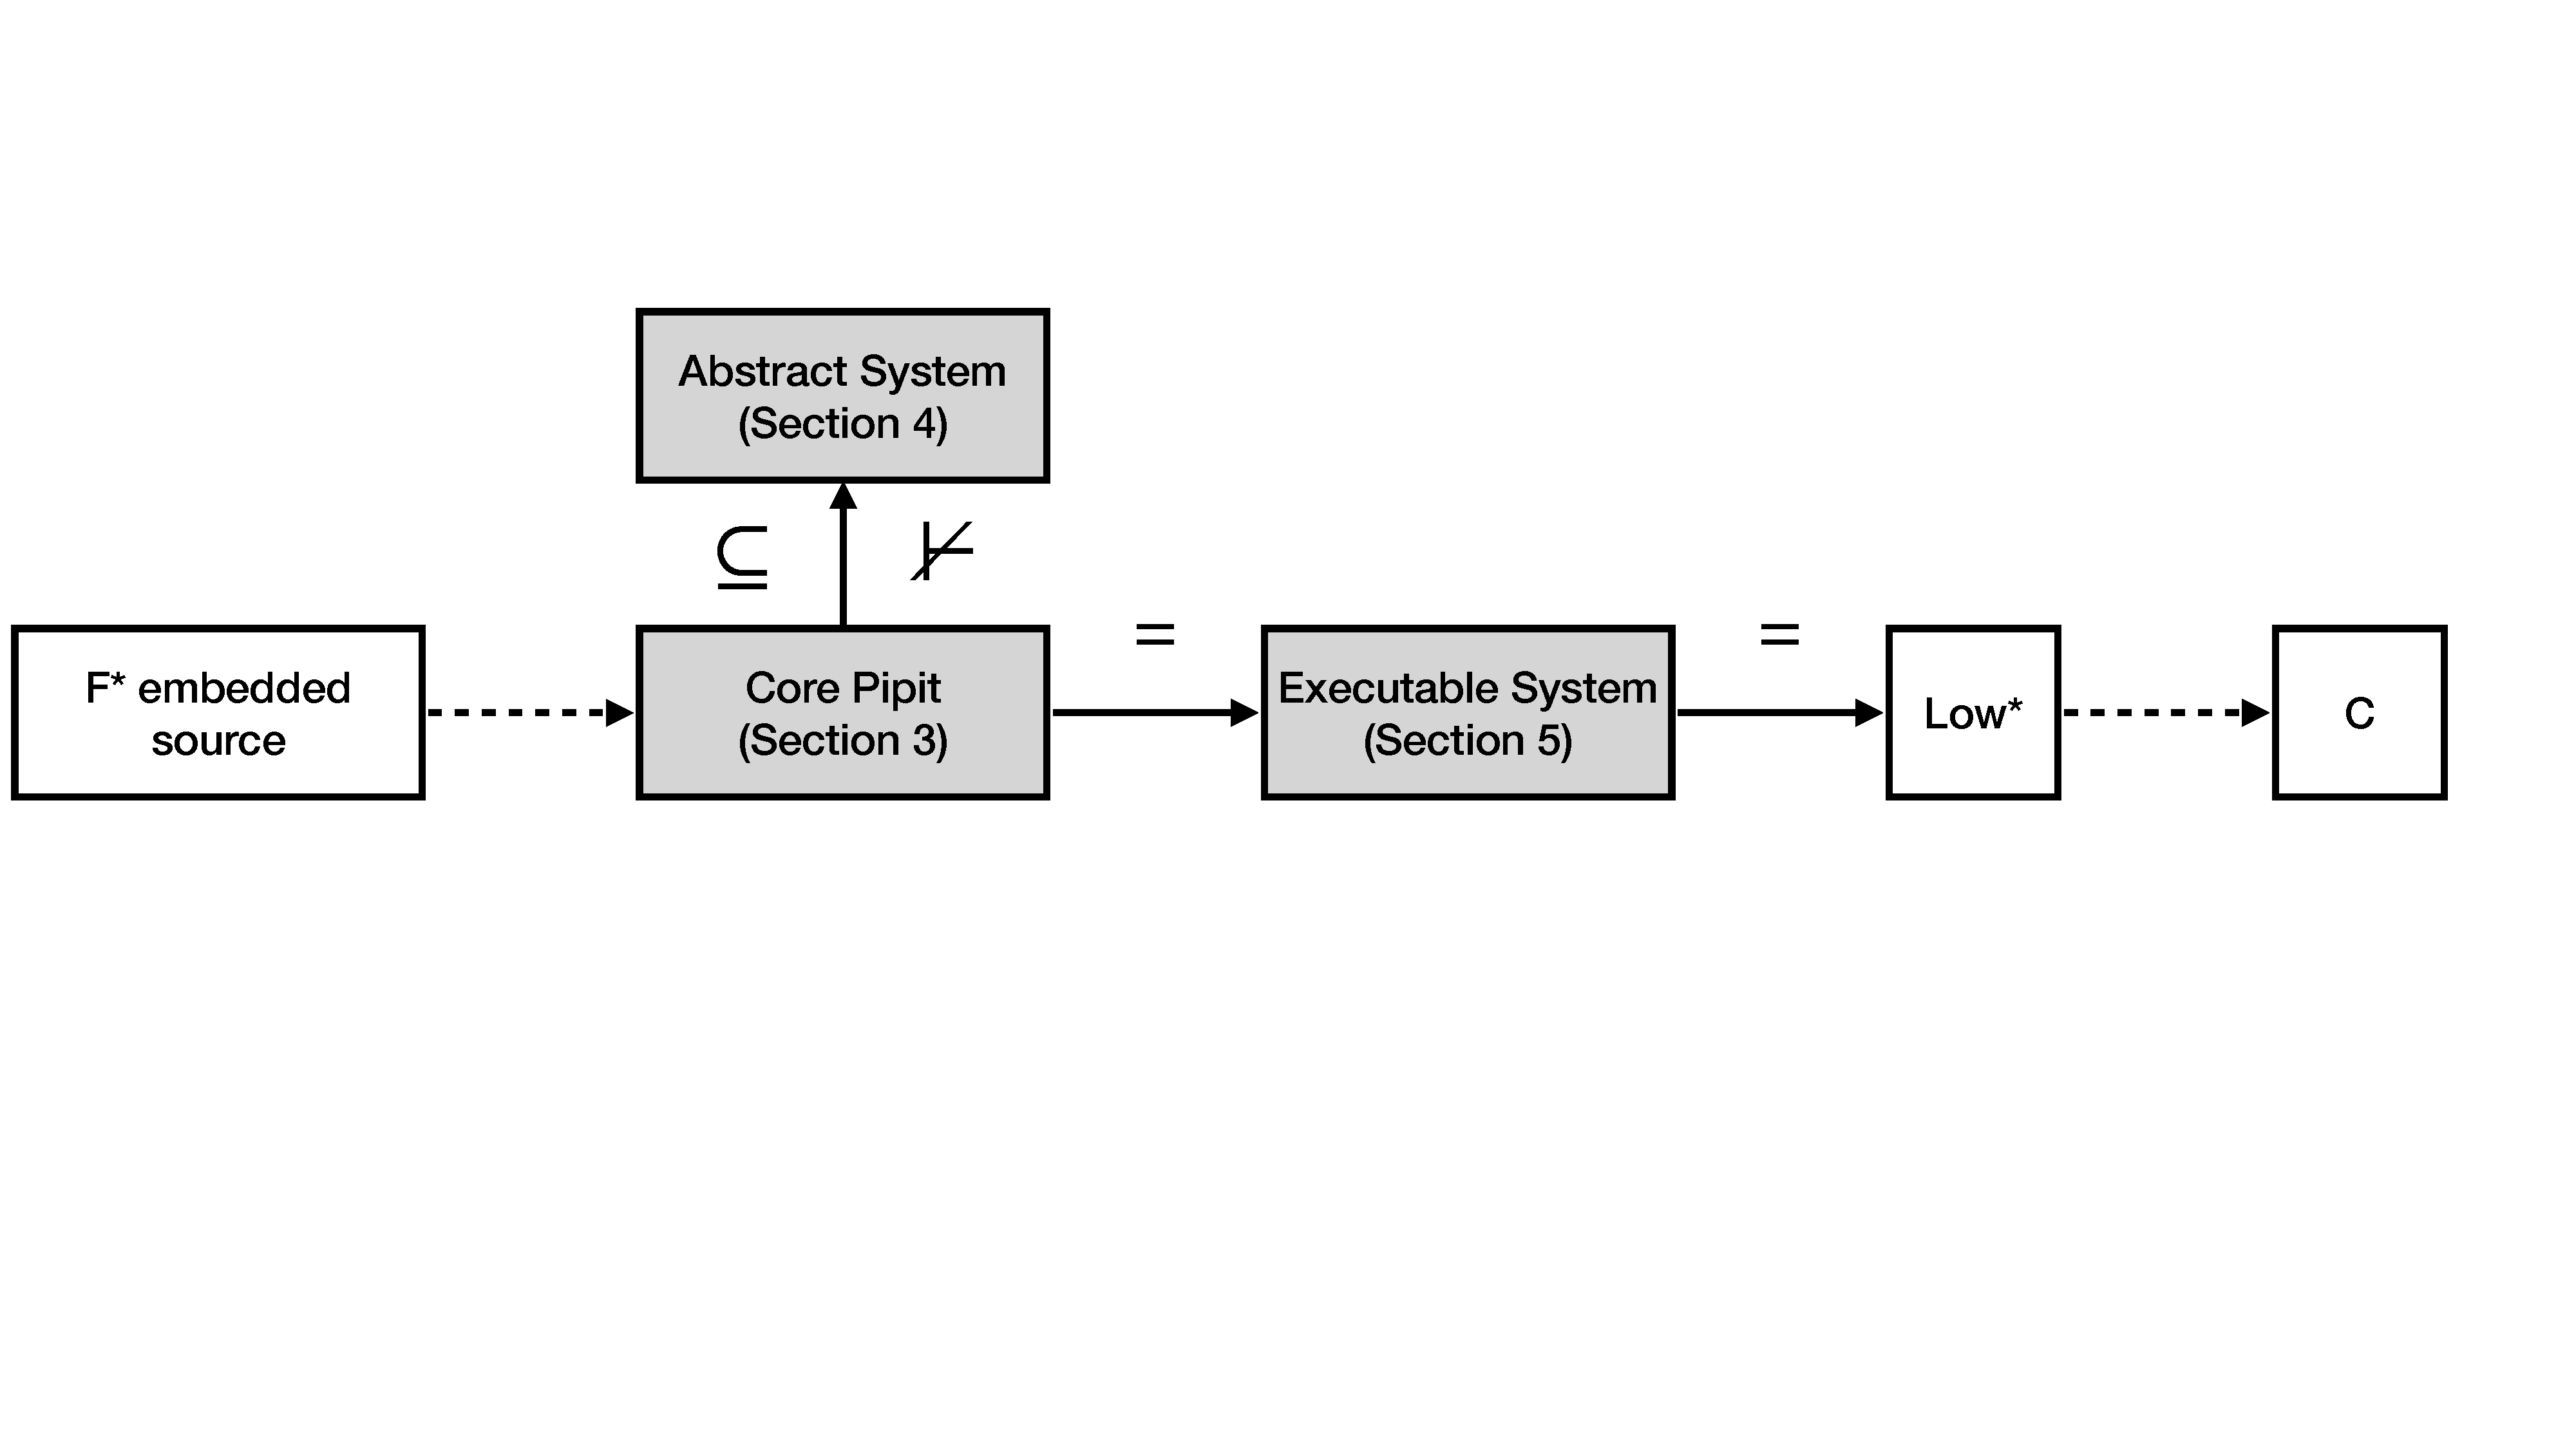
\includegraphics[width=\textwidth]{figures/core-structure.pdf}
\caption{Architecture of Pipit. The gray boxes and solid arrows are defined in this paper. The white boxes and dashed arrows are trusted components. The labels next to the arrows denote properties of the translation.
}
\label{f:core:structure}
\end{figure}
 
We now introduce the core Pipit language.
Note that this form differs slightly from the surface syntax presented earlier in \autoref{s:motivation}, which used the syntax of the metalanguage \fstar{}, as well as including proofs in \fstar{} itself.


\autoref{f:core:structure} shows the high-level architecture of Pipit.
On the left-hand-side, the surface syntax embedded in \fstar{} is shown; this includes some Pipit-specific syntactic sugar.
The translation from the surface syntax to the core language is trusted.
There are two targets from the core language: abstract transition systems for verification, and executable transition systems for extraction to C.
The translation to abstract systems is verified to be an abstraction according to the dynamic semantics (\autoref{s:core:dynamic}).
One property that still remains to be proven is that the proof obligations on the abstract transition system entail the original proof obligations (\autoref{s:transition}); this pending proof is denoted as negated entailment in the figure ($\not\vdash$).
The translation to executable transition system is proven to be semantics preserving, as is the subsequent translation to \lowstar{}.
The translation from \lowstar{} to C is external to this paper and forms part of our trusted computing base.


\autoref{f:core-grammar} defines the grammar of Pipit.
The expression form $e$ includes standard syntax for values ($v$), variables ($x$) and primitive applications ($p(\ov{e})$).
Most of the expression forms were introduced informally in \autoref{s:motivation} and correspond to the clock-free expressions of Lustre~\cite{caspi1995functional}.



\begin{figure}
  \[
  \begin{array}{lrlr}
    e, e' & := & v ~|~ x ~|~ p(\ov{e}) & \mbox{(values, variables and operations)} \\
          & | & \xfby{v}{e} ~|~ \xrec{x}{e[x]} & \mbox{(delayed and recursive streams)} \\ & | & \xlet{x}{e}{e'[x]} & \mbox{(let-expressions)}\\
          & | & \xcheckP{\PStatus}{e_{\text{prop}}} & \mbox{(checked properties)} \\
          & | & \xcontractP{\PStatus}{\erely}{\ebody}{\rawbind{x}{\eguar[x]}} & \mbox{(rely-guarantee contracts)} \\
\\
    v & := & n \in \mathbb{N} ~|~ b \in \mathbb{B} ~|~ r \in \mathbb{R} ~|~ \hdots  & \mbox{(values)} \\
    p & := & (+) ~|~ (-) ~|~ (\times) ~|~ \tt{if-then-else} ~|~ \hdots & \mbox{(primitives)} \\
    \\
    \PStatus & := & \PSValid ~|~ \PSUnknown & \mbox{(property statuses: valid or unknown)}\\
    \\
    V & := & \cdot ~|~ V;v & \mbox{(streams of values)} \\
    \sigma & := & \sgl{\ov{x \mapsto v}} & \mbox{(heaps)} \\
    \Sigma & := & \cdot ~|~ \Sigma;\sigma & \mbox{(streaming history environments)} \\
\tau, \tau' & := & \mathbb{N} ~|~ \mathbb{B} ~|~ \tau \times \tau ~|~ \hdots & \mbox{(value types)} \\
    \Gamma & := & \cdot ~|~ x : \tau, \Gamma & \mbox{(type environments)}  \\
    \end{array}
  \]
  \caption{Pipit core language grammar, which contains expressions $e$, values $v$, primitive operations $p$, and property statuses $\PStatus$.}
  \label{f:core-grammar}
\end{figure} 
The expression syntax for delayed streams ($\xfby{v}{e}$) denotes the previous value of the stream $e$, with an initial value of $v$ when there is no previous value.


Recursive streams, which can refer to previous values of the stream itself, are defined using the fixpoint operator ($\xrec{x}{e[x]}$); the syntax $e[x]$ means that the variable $x$ can occur in $e$.
As in Lustre, recursive streams can only refer to their previous values and must be \emph{guarded} by a delay: the stream $(\xrec{x}{\xfby{0}{(x + 1)}})$ is well-defined, but stream $(\xrec{x}{x + 1})$ is invalid and has no computational interpretation.
This form of recursion differs slightly from standard Lustre, which uses a set of mutually-recursive bindings.
Although we cannot express mutually-recursive bindings in the core syntax here, we can express them as a notation on the surface syntax by combining the bindings together into a record or tuple.

Checked properties and contracts are annotated with their property status $\PStatus$, which can either be valid ($\PSValid$) or unknown ($\PSUnknown$).
For checked properies $\xcheckP{\PStatus}{e}$, the property status denotes whether the property has been proved to be valid.

Contracts $\xcontractP{\PStatus}{\erely}{\ebody}{\rawbind{x}\eguar[x]}$ involve two verification conditions.
Firstly, when a contract is \emph{defined}, the definer must prove that the body satisfies the contract: roughly, if $\erely$ is always true, then $\eguar[x := \ebody]$ is always true.
Secondly, when a contract is \emph{instantiated}, the caller must prove that the environment satisfies the precondition: that is, $\erely$ is always true.
Conceptually, then, a contract could have two property statuses: one for the definition and one for the instantiation.
However, in practice, it is not useful to defer the proof of a contract definition --- one could achieve a similar effect by replacing the contract with its implementation.
For this reason, we only annotate contracts with one property status, which denotes whether the instantiation has been proved to satisfy the precondition.

For the presentation of the formal grammar here, we consider only a fixed set of values and primitives; in practice, the implementation is parameterised by a primitive table which we extend with immutable array operations for the TTCAN driver logic in \autoref{s:evaluation}.

Streams $V$ are represented as a sequence of values; streaming history environments $\Sigma$ are streams of heaps.
Types $\tau$ and type environments $\Gamma$ are standard.



\begin{figure}
  \begin{mathpar}
    \boxed{\typing{\Gamma}{e}{\tau}}
\end{mathpar}

  \begin{mathpar}
    \ruleIN{
      \mtypingval{v}{\tau}
    }{
      \typing{\Gamma}{v}{\tau}
    }{TValue}

    \ruleAx{\typing{\Gamma, x: \tau, \Gamma'}{x}{\tau}}{TVar}

    \ruleIN{
      \mtypingprim{p}{(\tau_1 \times \dots \times \tau_n) \to \tau'}
      \qquad
      \typing{\Gamma}{e_1}{\tau_1}
      \quad \hdots \quad
      \typing{\Gamma}{e_n}{\tau_n}
    }{\typing{\Gamma}{p(\ov{e})}{\tau'}}{TPrim}

    \ruleIN{
      \mtypingval{v}{\tau}
      \qquad
      \typing{\Gamma}{e'}{\tau}
    }{
      \typing{\Gamma}{\xfby{v}{e'}}{\tau}
    }{TFby}

\ruleIN{
      \typing{\Gamma, x : \tau}{e}{\tau}
    }{
      \typing{\Gamma}{\xrec{x}{e[x]}}{\tau}
    }{TRec}

    \ruleIN{
      \typing{\Gamma}{e}{\tau}
      \qquad
      \typing{\Gamma, x : \tau}{e'}{\tau'}
    }{
      \typing{\Gamma}{\xlet{x}{e}{e'[x]}}{\tau'}
    }{TLet}

    \ruleIN{
      \typing{\Gamma}{e}{\mathbb{B}}
    }{
      \typing{\Gamma}{\xcheckP{\PStatus}{e}}{\tt{unit}}
    }{TCheck}
  \and
    \ruleIN{
      \typing{\Gamma}{\erely}{\mathbb{B}}
      \qquad
      \typing{\Gamma}{\ebody}{\tau}
      \qquad
      \typing{\Gamma, x: \tau}{\eguar}{\mathbb{B}}
    }{
      \typing{\Gamma}{\xcontractP{\PStatus}{\erely}{\ebody}{\rawbind{x}{\eguar[x]}}}{\tau}
    }{TContract}
  \end{mathpar}

  \caption{Typing rules for Pipit; the judgment $\typing{\Gamma}{e}{\tau}$ denotes that expression $e$ describes a \emph{stream} of values of type $\tau$. Two auxiliary functions are used for values and primitive operations; their definitions are standard and are omitted.}\label{f:core-typing}
\end{figure} 
We define the typing judgments for Pipit in \autoref{f:core-typing}.
Most of the typing rules are standard for an unclocked Lustre.
The typing judgment $\typing{\Gamma}{e}{\tau}$ denotes that, in an environment of streams $\Gamma$, expression $e$ denotes a stream of type $\tau$.
This core typing judgment differs from the surface syntax used in \autoref{s:motivation}, which used an explicit stream type; for the core language, we instead assume that everything is a stream.

For values, we use an auxiliary definition $\mtypingval{v}{\tau}$ to denote that value $v$ has type $\tau$.
Likewise, for primitives we use $\mtypingprim{p}{(\tau_1 \times \cdots \hdots \times \tau_n) \to \tau'}$ to denote that primitive $p$ takes arguments of type $\tau_i$ and returns a result of type $\tau'$.
Primitives are pure, non-streaming functions.

Rules \textsc{TValue}, \textsc{TVar}, \textsc{TPrim} and \textsc{TLet} are standard.

Rule \textsc{TFby} states that expression $\xfby{v}{e}$ requires both $v$ and $e$ to have equal types; the result is the same type.

Rule \textsc{TRec} states that a recursive stream $\xrec{x}{e}$ has the recursive stream bound inside $e$.
The recursion must also be guarded, in that any recursive references to $x$ are delayed, but this requirement is performed as a separate syntactic check described in \autoref{s:core:causality}.

Rule \textsc{TCheck} states that statically checking a property $\xcheckP{\PStatus}{e}$ requires a boolean property $e$ and returns unit.

Finally, rule \textsc{TContract} applies for a contract $\xcontractP{\PStatus}{\erely}{\ebody}{\rawbind{x}\eguar[x]}$ with a body expression of some type $\tau$.
The overall expression has result type $\tau$.
Both rely and guarantee clauses must be boolean expressions.
Additionally, the guarantee clause can refer to the result value as $x$.

\subsection{Dynamic semantics}
\label{s:core:dynamic}


\begin{figure}
  \begin{mathpar}
    \boxed{\bigstep{\Sigma}{e}{v}}
  \end{mathpar}

  \begin{mathpar}
    \ruleAx{\bigstep{\Sigma}{v}{v}}{Value}
    \quad
    \ruleAx{\bigstep{\Sigma; \sigma}{x}{\sigma(x)}}{Var}

    \ruleIN{
      \bigstep{\Sigma}{e_1}{v_1} \quad \hdots \quad
      \bigstep{\Sigma}{e_n}{v_n}
    }{\bigstep{\Sigma}{p(\ov{e})}{\text{prim-sem}(p, \ov{v})}}{Prim}



  \ruleAx{\bigstep{\sigma}{\xfby{v}{e'}}{v}}{$\mbox{Fby}_1$}
    \quad
    \ruleIN{\text{length}(\Sigma) > 0 \and \bigstep{\Sigma}{e'}{v'}}{\bigstep{\Sigma; \sigma}{\xfby{v}{e'}}{v'}}{$\mbox{Fby}_S$}



    \ruleIN{
      \bigstep{\Sigma}{e[x := \xrec{x}{e}]}{v}
    }{
      \bigstep{\Sigma}{\xrec{x}{e[x]}}{v}
    }{Rec}

    \ruleIN{
      \bigstep{\Sigma}{e'[x := e]}{v}
    }{
      \bigstep{\Sigma}{\xlet{x}{e}{e'[x]}}{v}
    }{Let}

    \ruleIN{
}{
      \bigstep{\Sigma}{\xcheckP{\PStatus}{e}}{()}
    }{Check}

    \ruleIN{
      \bigstep{\Sigma}{\ebody}{v}
    }{
      \bigstep{\Sigma}{\xcontractP{\PStatus}{\erely}{\ebody}{\rawbind{x}{\eguar[x]}}}{v}
    }{Contract}
  \end{mathpar}


  \begin{mathpar}
    \boxed{\bigsteps{\Sigma}{e}{V}}

    \boxed{\bigstepalways{\Sigma}{e}}
  \end{mathpar}

  \begin{mathpar}
    \ruleAx{\bigsteps{\cdot}{e}{\cdot}}{$\mbox{Steps}_0$}


    \ruleIN{
      \bigstep{\Sigma}{e}{V}
      \and
      \bigstep{\Sigma; \sigma}{e}{v}
    }{\bigstep{\Sigma; \sigma}{e}{V; v}}{$\mbox{Steps}_S$}

    \ruleIN{\bigsteps{\Sigma}{e}{\true; \hdots}}{\bigstepalways{\Sigma}{e}}{Always}
  \end{mathpar}


  \caption{Dynamic semantics for Pipit; the judgment form $\bigstep{\Sigma}{e}{v}$ denotes that evaluating expression $e$ under streaming history $\Sigma$ results in value $v$.}\label{f:core-bigstep}
\end{figure}
 
The dynamic semantics of Pipit are defined in \autoref{f:core-bigstep}.
We present our semantics in a big-step form.
This differs somewhat from traditional \emph{reactive} semantics of Lustre~\cite{caspi1995functional}.
Our big-step semantics emphasises the equational nature of Pipit, as it is substitution-based and syntax-directed, while the reactive semantics emphasises the finite-state streaming execution of the system.
We use transition systems for reasoning about the finite-state execution (\autoref{s:transition}), which is fairly standard~\cite{brun2023equation,champion2016kind2,raymond2008synchronous}.
Previous work on the {\sc W-calculus}~\cite{gallego2021w} for linear digital-signal-processing filters makes a similar distinction and provides a non-streaming semantics for reasoning about programs and a streaming semantics for executing programs.


The judgment form $\bigstep{\Sigma}{e}{v}$ denotes that expression $e$ evaluates to value $v$ under streaming history $\Sigma$.
The streaming history is a stream of heaps; in practice, we only evaluate expressions with a non-empty streaming history.

Rule {\sc Value} states that evaluating a value results in the value itself.

Rule {\sc Var} states that to evalute a variable $x$ under some non-empty stream history $\Sigma; \sigma$, where $\sigma$ is the most recent heap, we look up the variable in $\sigma$.

Rule {\sc Prim} states that to evaluate a primitive $p$ applied to many arguments $e_1$ to $e_n$, we evaluate each argument separately; we then apply the primitive with prim-sem metafunction.

Rule $\textsc{Fby}_1$ evaluates a followed-by expression when the streaming history contains only a single element.
Here, $\xfby{v}{e}$ evaluates to $v$, as there is no previous value of $e$ to use.

Rule $\textsc{Fby}_S$ evaluates a followed-by expression when the streaming history contains multiple entries.
In this case, $\xfby{v}{e}$ evaluates the previous value of $e$ by discarding the most recent entry from the streaming history.

Rule {\sc Rec} evaluates a recursive stream $\xrec{x}{e}$ by unfolding the recursion one step.
For causal expressions (\autoref{s:core:causality}), where each recursive occurrence of $x$ is guarded by a followed-by, this unfolding eventually terminates as each followed-by shortens the history.

Rule {\sc Let} is standard.

Rule {\sc Check} states that check expressions always evaluate to unit.
We do not perform a dynamic check that the property is true here; checking the truth of properties is dealt with in the checked semantics (\autoref{s:core:checked}).

Rule {\sc Contract} states that contracts evaluate by just evaluating their body.
Like with checks, we do not perform a dynamic check that the precondition and postcondition hold.


We also define two auxiliary judgment forms: $\bigsteps{\Sigma}{e}{V}$ and $\bigstepalways{\Sigma}{e}$.

Judgment form $\bigsteps{\Sigma}{e}{V}$ denotes that, under history $\Sigma$, expression $e$ evaluates to the \emph{stream} $V$.
This judgment performs iterated application of single-value evaluation.

Judgment form $\bigstepalways{\Sigma}{e}$ denotes that a boolean expression $e$ evaluates to the stream of trues under history $\Sigma$.
Informally, it can be read as ``$e$ is always true in history $\Sigma$''.

\subsection{Checked semantics}
\label{s:core:checked}


\begin{figure}
  \begin{mathpar}
    \boxed{\semcheck{\Sigma}{\PStatus}{e}}
  \end{mathpar}

  \begin{mathpar}
    \ruleAx{\semcheck{\Sigma}{\PStatus}{v}}{ChkValue}
    \quad
    \ruleAx{\semcheck{\Sigma}{\PStatus}{x}}{ChkVar}

    \ruleIN{
      \semcheck{\Sigma}{\PStatus}{e_1} \quad \hdots \quad
      \semcheck{\Sigma}{\PStatus}{e_n}
    }{\semcheck{\Sigma}{\PStatus}{p(\ov{e})}}{ChkPrim}


  \ruleAx{\semcheck{\sigma}{\PStatus}{\xfby{v}{e'}}}{$\mbox{ChkFby}_1$}

    \ruleIN{\text{length}(\Sigma) > 0 \and \semcheck{\Sigma}{\PStatus}{e'}}{\semcheck{\Sigma; \sigma}{\PStatus}{\xfby{v}{e'}}}{$\mbox{ChkFby}_S$}

    \ruleIN{
      \semcheck{\Sigma}{\PStatus}{e[x := \xrec{x}{e}]}
    }{
      \semcheck{\Sigma}{\PStatus}{\xrec{x}{e[x]}}
    }{ChkRec}

    \ruleIN{
      \semcheck{\Sigma}{\PStatus}{e'[x := e]}
    }{
      \semcheck{\Sigma}{\PStatus}{\xlet{x}{e}{e'[x]}}
    }{ChkLet}

    \ruleIN{
      (\PStatus = \PStatus' \implies \bigstepalways{\Sigma}{e})
      \and
      \semcheck{\Sigma}{\PStatus}{e}
    }{
      \semcheck{\Sigma}{\PStatus}{\xcheckP{\PStatus'}{e}}
    }{ChkCheck}



    \inferrule{
      (\PStatus = \PStatus' \implies \bigstepalways{\Sigma}{\erely})
      \\\\
      (\PStatus = \PSValid \implies \bigstepalways{\Sigma}{\erely} \implies \bigstepalways{\Sigma}{\eguar[x := \ebody]})
      \\\\
      \semcheck{\Sigma}{\PStatus}{\erely}
      \\\\
      (\bigstepalways{\Sigma}{\erely} \implies \semcheck{\Sigma}{\PStatus}{\ebody} ~\wedge~ \semcheck{\Sigma}{\PStatus}{\eguar[x := \ebody]})
    }{
      \semcheck{\Sigma}{\PStatus}{\xcontractP{\PStatus'}{\erely}{\ebody}{\rawbind{x}{\eguar[x]}}}
    }(\textsc{ChkContract})

\end{mathpar}

  \caption{Checked semantics for Pipit; the judgment form $\semcheck{\Sigma}{\PStatus}{e}$ denotes that evaluating expression $e$ under streaming history $\Sigma$ satisfies the checks and rely-guarantee contract requirements that are labelled with property status $\PStatus$.}\label{f:core-check}
\end{figure}
 
In addition to the big-step semantics above, we also define a judgment form for checking that the properties and contracts of a program hold for a particular streaming history.
We call these the \emph{checked} semantics.
Unlike an axiomatic semantics, the checked semantics operate on a concrete set of input streams.

The checked semantics have the judgment form $\semcheck{\Sigma}{\PStatus}{e}$, which denotes that under streaming history $\Sigma$, the properties of $e$ with status $\PStatus$ hold.
The property status dictates which properties should be checked and which should be ignored.

To show that an expression $e$'s unknown properties hold, we prove that for all streaming histories $\Sigma$, assuming the valid properties hold ($\semcheck{\Sigma}{\PSValid}{e}$), then the unknown properties ($\semcheck{\Sigma}{\PSUnknown}{e}$) hold.
The assumption here means that we do not have to re-check properties after proving them once.

Contracts involve two proofs: one for the definition and one for the instantiation.
To prove that a contract definition $\xcontractP{\PStatus}{\erely}{\ebody}{\rawbind{x}\eguar[x]}$ is valid, we show that for all streaming histories $\Sigma$, assuming the rely is always true under the history ($\bigstepalways{\Sigma}{\erely}$), then the body always satisfies the guarantee ($\bigstepalways{\Sigma}{\eguar[x := \ebody]}$).
Additionally, we can also assume that the valid properties in all three components hold, and we must also show that the unknown properties are valid.
The fact that the checked semantics refers to a particular $\Sigma$ is significant here: it allows the proof of contract validity to only consider streaming histories where the rely actually holds.



To prove that a contract \emph{instantiation} (a call-site) is valid, we show that, under the calling environment, the rely clause is always true.
Crucially, the proof can also use the fact that, if the rely is always true, then the guarantee is always true.
This sort of feedback is necessary for proving properties of mutually-dependent calls.
This circular dependency is well-founded as our causality check ensures that recursive streams are guarded by delays (\autoref{s:core:causality}).

We define the checked semantics of Pipit in \autoref{f:core-check}.
The checked semantics mostly follows the structure of the dynamic semantics, additionally checking any properties and contracts as they are encountered.

Rules {\sc ChkValue} and {\sc ChkVar} state that values and variables are always valid.

Rule {\sc ChkPrim} checks a primitive application by descending into the subexpressions.

Rules $\textsc{ChkFby}_1$ and $\textsc{ChkFby}_S$ are derived from the structure of the big-step rules  $\textsc{Fby}_1$ and $\textsc{Fby}_S$.
At an input stream of length one, $\textsc{ChkFby}_1$ asserts that all subproperties hold for the (non-existent) previous values in the stream.
At subsequent parts of the stream, $\textsc{ChkFby}_S$ discards the most recent element of the stream history and checks the subexpression with the previous inputs.


Rules {\sc ChkRec} and {\sc ChkLet} both perform the same unfolding as the corresponding big-step rules and check the resulting expression.

Finally, the heavy lifting is performed by rules {\sc ChkCheck} and {\sc ChkContract}.

Rule {\sc ChkCheck} applies when checking property status $\PStatus$ of an expression $\xcheckP{\PStatus'}{e}$.
If the check-expression has the same status as what we are checking ($\PStatus = \PStatus'$), then we perform the actual check by evaluating the expression $e$ and requiring it to evaluate to a stream of trues.
Otherwise, we do not need to evaluate the check-expression.
In both cases, we descend into the expression and check its subexpressions, as they may have nested properties.
Such nested properties are unlikely to be written directly by the user, but might occur after program transformations such as inlining.

Rule {\sc ChkContract} applies when checking property status $\PStatus$ of a contract with expression $\xcontractP{\PStatus'}{\erely}{\ebody}{\rawbind{x}\eguar[x]}$.
Although we only include one property status on the contract, conceptually there are two distinct properties: one for the caller ($\PStatus'$) and one for the definition itself (assumed to be $\PSValid$).
To check the caller property when $\PStatus = \PStatus'$, we evaluate the rely $\erely$ and require it to be true.
To check the definition property when $\PStatus = \PSValid$, we assume that the rely holds, and check that the body satisfies the guarantee.
We also descend into the subexpressions to check them; when checking the body and guarantee, we can assume that the rely holds.


\subsubsection{Blessing expressions and contracts}
\label{s:core:blessing}

Blessing is a meta-operation that replaces the property statuses in an expression so that all checks and contracts are marked as valid ($\PSValid$).
Blessing an expression requires a proof that the checked semantics hold for all input streams:

$$
\ruleIN{
  \forall \Sigma.~
  \semcheck{\Sigma}{\PSValid}{e}
  \implies
  \semcheck{\Sigma}{\PSUnknown}{e}
}{\text{bless}~e}{BlessExpression}
$$

Blessing is different for contract definitions, as we need to separate the definition of the contract from the instantiation.
To check that a contract definition is valid, we show that if the rely clause is always true for a particular input, then the body satisfies the guarantee for the same inputs.
We also assume that the valid properties in the rely, body and guarantee hold, and show the corresponding unknown properties:

\begin{tabbing}
  \tt{MM}\= \tt{MMMM} \= \tt{MMMMMMMMMMMMM} \= \kill
  \tt{let} $\text{contract_valid}~\{ \erely \} ~\ebody~ \{ \eguar \}: \text{prop}$ = \\
  \> $\forall \Sigma.$
  \> $ (
    \semcheck{\Sigma}{\PSValid}{(\erely, \ebody, \eguar[x := \ebody])}
    ~\wedge~
    \bigstepalways{\Sigma}{\erely}
  ) $ \\
  \> $\implies$
  \> $(
    \semcheck{\Sigma}{\PSUnknown}{(\erely, \ebody, \eguar[x := \ebody])}
    ~\wedge~
    \bigstepalways{\Sigma}{\eguar[x := \ebody]}
    )$
\end{tabbing}

After proving that the contract is valid for all inputs, we can bless the contract definition.
Blessing the contract definition blesses the subexpressions for the rely, body and guarantee, but leaves the contract's \emph{instantiation} property status as unknown:
$$
\inferrule{
  \text{contract_valid}~\{ \erely \} ~\ebody~ \{ \eguar \}
}{\text{bless_contract}~\{\erely\}~\ebody~\{ \eguar\}}(\textsc{BlessContract})
$$




\subsection{Causality and metatheory}
\label{s:core:causality}

To ensure that recursive streams have a computational interpretation, we require that all recursive streams are guarded by a followed-by delay.
We implement this as a simple syntactic check: each $\xrec{x}{e}$ can only mention $x$ inside a followed-by.
This check is stricter than necessary: for example, the expression $\xrec{x}{(\xlet{x'}{x + 1}{\xfby{0}{x'}})}$ does mention the recursive stream $x$ outside of the delay, but after inlining the let, it would be causal.
We hope to relax this restriction somewhat in future work.

The causality restriction gives us some important properties about the metatheory.
The most important property is that the dynamic semantics form a total function: given a streaming history and a causal expression, we can evaluate the expression to a value.
These properties are mechanised in \fstar{}.



\begin{theorem}[bigstep-is-total]
  For any non-empty streaming history $\Sigma$ and causal expression $e$, there exists some value $v$ such that $e$ evaluates to $v$ $(\bigstep{\Sigma}{e}{v})$.
\end{theorem}

The relationship between substitution and the streaming history is also important.
In general, we have a substitution property that states that evaluating a substituted expression $e[x := e']$ under some context $\Sigma$ is equivalent to evaluating $e'$ and adding it to the context $\Sigma$:

\begin{theorem}[bigstep-substitute]
  For a streaming history $\Sigma$ and causal expressions $e$ and $e'$, if $e[x := e']$ evaluates to a value $v$ $(\bigstep{\Sigma}{e}{v})$, then we can evaluate $e'$ to some stream $V$ and extend the streaming history to evaluate $e$ to the original value $(\bigstep{\Sigma[x \mapsto V]}{e}{v})$.
  The converse is also true.
\end{theorem}



The semantics in \autoref{f:core-bigstep} for a recursive expression $\xrec{x}{e}$ performs one step of recursion by substituting $x$ for the recursive expression.
An alternative non-syntax-directed semantics would be to have the environment outside the semantics supply a stream $V$ such that if we extend the streaming history with $x \mapsto V$, then $e$ evaluates to $V$ itself.
The above substitution theorem can be used to show that, for causal expressions, these two semantics are equivalent.
We can additionally show that, when evaluating $e$ with $x \mapsto V$, the most recent value in $V$ does not affect the result.
This fact can be used to ``seed'' evaluation by starting with an arbitrary value:
\begin{theorem}[bigstep-rec-causal]
  For a streaming history $\Sigma; \sigma$ and a causal recursive expression $\xrec{x}{e}$, if $(\bigstep{\Sigma; \sigma}{e}{v})$, then updating $\sigma[x]$ with any value $v'$ results in the same value: $(\bigstep{\Sigma; \sigma[x \mapsto v']}{e}{v})$.
\end{theorem}

 







 

\section{Abstract transition systems}
\label{s:transition}


\begin{figure}
  \begin{tabbing}
  MM \= update: \= \kill
  \tt{type} system (input: $\Gamma$) (result: $\tau$) = \{ \\
  \> state:  \> $\Gamma$; \\
  \> free: \> $\Gamma$; \\
  \> init: \> heap state; \\
  \> step: \> heap input $\to$ heap free $\to$ heap state $\to$ step_result state result; \\
  \} \\
  \\
  \tt{type} step_result (state: $\Gamma$) (result: $\tau$) = \{ \\
  \> update:  \> heap state; \\
  \> value: \> result; \\
  \> rely: \> \tt{prop}; \\
  \> guar: \> \tt{prop}; \\
  \}
  \end{tabbing}
  \caption{Abstract transition system type definitions}
  \label{f:system-types}
\end{figure} 
To prove properties about Pipit programs, we translate to an \emph{abstract} transition system, so-called because it abstracts away the implementation details of contract instantiations.
For extraction we also translate to \emph{executable} transition systems, which we discuss in \autoref{s:extraction}.

\autoref{f:system-types} shows the types of transition systems.
A transition system is parameterised by its input context and the result type.
It also contains two internal contexts: firstly, the state context describes the private state required to execute the machine; secondly, the free context contains any extra input values that the transition system would like to existentially quantify over.
The free context is used to allow the system to ask for arbitrary values from the environment, when it would not otherwise be able to return a concrete value.

For contract instantiations, which abstract over the implementation, the natural translation to a transition system would involve an existential quantifier: ``there exists some value that satisfies the specification''.
Unfortunately, such an existential quantifier requires a step \emph{relation} rather than a step \emph{function}.
Using a step relation complicates the resulting transition system, as other operations such as primitive application must also introduce existential quantifiers; such quantifiers block simplifications such as partial-evaluation and result in a more complex transition system.
Instead, the free context provides the step function with a fresh unconstrained value of the desired type, which the step function can then constrain.

Back to \autoref{f:system-types}, the step-result contains the updated state for the transition system, as well as the result value.
The step-result additionally contains two propositions for the `rely', or assumptions about the execution environment, and `guarantee', or obligations that the transition system must show.
For the transition system corresponding to an expression $e$, these propositions are analogous to the known checked semantics $\semcheck{\Sigma}{\PSValid}{e}$ and unknown checks $\semcheck{\Sigma}{\PSUnknown}{e}$ respectively.

Our implementation includes a mechanised proof that, for causal expressions, the transition system is an abstraction of the original expression's dynamic semantics.
The proof that the rely and guarantee propositions correspond to the checked semantics is future work.







\newcommand{\sysinit}[1]{\systrans{#1}_{\text{init}}}
\newcommand{\sysvalue}[1]{\systrans{#1}_{\text{value}}}
\newcommand{\sysupdate}[1]{\systrans{#1}_{\text{update}}}
\newcommand{\sysrely}[1]{\systrans{#1}_{\text{rely}}}
\newcommand{\sysguar}[1]{\systrans{#1}_{\text{guar}}}
\newcommand{\xctr}{\xcontractP{\PStatus}{e_r}{e_b}{\rawbind{x}{e_g}}}

\newcommand{\sysstate}[1]{\systrans{#1}_{\text{state}}}
\newcommand{\sysoracle}[1]{\systrans{#1}_{\text{free}}}

\begin{figure}
  \small
  \[
  \begin{array}{rrlr}
    \sysstate{v} & = & \cdot \\
    \sysstate{x} & = & \cdot \\
    \sysstate{p(\ov{e})} & = & \bigcup_i \sysstate{e_i} \\
    \sysstate{\xfby{v}{e}} & = & x_{\tt{fby}(e)}: \tau, \sysstate{e} & \text{(fresh $x_{\tt{fby}(e)}$)} \\
    \sysstate{\xrec{x}{e}} & = & \sysstate{e} \\
    \sysstate{\xlet{x}{e}{e'}} & = & \sysstate{e} \cup \sysstate{e'} \\
    \sysstate{\xcheckP{\PStatus}{e}} & = & \sysstate{e} \\
    \sysstate{\xctr} & = & \sysstate{e_r} \cup \sysstate{e_b} \\
    \\
    \sysoracle{v} & = & \cdot \\
    \sysoracle{x} & = & \cdot \\
    \sysoracle{p(\ov{e})} & = & \bigcup_i \sysoracle{e_i} \\
    \sysoracle{\xfby{v}{e}} & = & \sysoracle{e} \\
    \sysoracle{\xrec{x}{e}} & = & x: \tau, \sysoracle{e} \\
    \sysoracle{\xlet{x}{e}{e'}} & = & \sysoracle{e} \cup \sysstate{e'} \\
    \sysoracle{\xcheckP{\PStatus}{e}} & = & \sysoracle{e} \\
    \sysoracle{\xctr} & = & x: \tau, \sysoracle{e_r} \cup \sysstate{e_b} \\
  \end{array}
\]
\caption{Transition system typing contexts of expressions; for an expression $e$, $\sysstate{e} : \Gamma$ and $\sysoracle{e} : \Gamma$ describe the heaps used to store the expression's internal state and extra inputs.}
\label{f:system-translation-contexts}
\end{figure}

\begin{figure}
  \small
  \[
  \begin{array}{lrl}
    \sysinit{v} & = & () \\
    \sysvalue{v}(i, f, s) & = & v \\
\\
    \sysinit{x} & = & () \\
    \sysvalue{x}(i, f, s) & = & (i \cup f).x \\
\\
    \sysinit{p(\ov{e})} & = & \bigcup_i \sysinit{e_i} \\
    \sysvalue{p(\ov{e})}(i, f, s) & = & \text{prim-sem}(p, \ov{\sysvalue{e}(i, f, s)}) \\
    \sysupdate{p(\ov{e})}(i, f, s) & = & \bigcup_i \sysupdate{e_i}(i, f, s) \\
    \sysrely{p(\ov{e})}(i, f, s) & = & \bigwedge_i \sysrely{e_i}(i, f, s) \\
    \sysguar{p(\ov{e})}(i, f, s) & = & \bigwedge_i \sysguar{e_i}(i, f, s) \\
    \\
    \sysinit{\xfby{v}{e}} & = & \sysinit{e} \cup \{ x_{\tt{fby}(e)} \mapsto v \} \\
    \sysvalue{\xfby{v}{e}}(i, f, s) & = & s.x_{\tt{fby}(e)} \\
    \sysupdate{\xfby{v}{e}}(i, f, s) & = & \sysupdate{e}(i, f, s) \cup \{x_{\tt{fby}(e)} \mapsto \sysvalue{e}(i, f, s)\}\\
    \sysrely{\xfby{v}{e}}(i, f, s) & = & \sysrely{e}(i, f, s) \\
    \sysguar{\xfby{v}{e}}(i, f, s) & = & \sysguar{e}(i, f, s) \\
    \\
    \sysinit{\xrec{x}{e}} & = & \sysinit{e} \\
    \sysvalue{\xrec{x}{e}}(i, f, s) & = & f.x \\
    \sysupdate{\xrec{x}{e}}(i, f, s) & = & \sysupdate{e}(i, f, s)\\
    \sysrely{\xrec{x}{e}}(i, f, s) & = & \sysrely{e}(i, f, s) \\
          & \wedge & f.x = \sysvalue{e}(i, f, s) \\
    \sysguar{\xrec{x}{e}}(i, f, s) & = & \sysguar{e}(i, f, s) \\
    \\
    \sysinit{\xlet{x}{e}{e'}} & = & \sysinit{e} \cup \sysinit{e'} \\
    \sysvalue{\xlet{x}{e}{e'}}(i, f, s) & = & \sysvalue{e'}(i \cup \{ x \mapsto \sysvalue{e}(i, f, s)\}, f, s) \\
    \sysupdate{\xlet{x}{e}{e'}}(i, f, s) & = & \sysupdate{e'}(i \cup \{ x \mapsto \sysvalue{e}(i, f, s)\}, f, s) \\
      & \cup & \sysupdate{e}(i, f, s) \\
    \sysrely{\xlet{x}{e}{e'}}(i, f, s) & = & \sysrely{e'}(i \cup \{ x \mapsto \sysvalue{e}(i, f, s)\}, f, s) \\
      & \wedge & \sysrely{e}(i, f, s) \\
    \sysguar{\xlet{x}{e}{e'}}(i, f, s) & = & \sysguar{e'}(i \cup \{ x \mapsto \sysvalue{e}(i, f, s)\}, f, s) \\
      & \wedge & \sysguar{e}(i, f, s) \\
    \\
    \sysinit{\xcheckP{\PStatus}{e}} & = & \sysinit{e} \\
    \sysvalue{\xcheckP{\PStatus}{e}}(i, f, s) & = & () \\
    \sysupdate{\xcheckP{\PStatus}{e}}(i, f, s) & = & \sysupdate{e}(i, f, s) \\
    \sysrely{\xcheckP{\PStatus}{e}}(i, f, s) & = & (\PStatus = \PSValid \implies \sysvalue{e}(i, f, s)) \wedge \sysrely{e}(i, f, s) \\
    \sysguar{\xcheckP{\PStatus}{e}}(i, f, s) & = & (\PStatus = \PSUnknown \implies \sysvalue{e}(i, f, s)) \wedge \sysguar{e}(i, f, s) \\
    \\
    \sysinit{\xctr} & = & \sysinit{e_r} \cup \sysinit{e_g} \\
    \sysvalue{\xctr}(i, f, s) & = & f.x \\
    \sysupdate{\xctr}(i, f, s) & = & \sysupdate{e_r}(i, f, s) \cup \sysupdate{e_g}(i, f, s) \\
    \sysrely{\xctr}(i, f, s) & = & (\sysvalue{e_r}(i, f, s) \implies \sysvalue{e_g}(i, f, s)) \\
                            & \wedge & (\PStatus = \PSValid \implies \sysvalue{e_r}(i, f, s)) \\
                            & \wedge & \sysrely{e_r}(i, f, s) \wedge \sysrely{e_g}(i, f, s) \\
    \sysguar{\xctr}(i, f, s) & = & (\PStatus = \PSUnknown \implies \sysvalue{e_r}(i, f, s)) \\
    & \wedge & \sysguar{e_r}(i, f, s) \wedge \sysguar{e_g}(i, f, s) \\
\end{array}
  \]
  \caption{Transition system semantics; for an expression $\Gamma \vdash e: \tau$, $\sysinit{e} : \text{heap~}\sysstate{e}$ is the initial state. For each field of the step-result type, we define a translation function that takes the input, free and state heaps: for example, we define the value-result of a step with type $\sysvalue{e}: \text{heap~}\Gamma \to \text{heap~}\sysoracle{e} \to \text{heap~}\sysstate{e} \to \tau$.}
  \label{f:system-translation}
\end{figure} 
\autoref{f:system-translation-contexts} defines the internal state and free contexts required for an expression.
For most expression forms, the state and free contexts are defined by taking the union of the contexts of subexpressions.
Followed-by delays introduce a local state variable $x_{\tt{fby}(e)}$ in which to store the most recent stream value.
We generate a fresh variable here, though the implementation uses de Bruijn indices.
Recursive streams and contracts both introduce new bindings into the free context; we assume that their binders $x$ are unique.

\autoref{f:system-translation} defines the translation for expressions.
Values and expressions have no internal state.
For variables, we look for the variable binding in either of the input or free heaps; bindings are unique and cannot occur in both.
We omit the rely and guarantee definitions here; both are trivially true.

To translate primitives, we union together the initial states of the subexpressions; updating the state is similar.
For the rely and guarantee definitions, we take the conjunction: we can assume that all subexpressions rely clauses hold, and must show that all guarantees hold.

To translate a followed-by $\xfby{v}{e}$, we initialise the follow-by's unique binder $x_{\tt{fby}(e)}$ to $v$.
At each step, we return the value in the local state, before updating the local state to the subexpression's new value.
The rely and guarantee differ from the checked semantics here: in the checked semantics, we check the subexpression on the previous inputs, but here we check the current subexpression.
This means that a single step of the rely and guarantee do not exactly correspond to the checked semantics; however, we posit that they are equivalent for a rely and guarantee that has been proven to hold for any sequence of inputs.

To translate a recursive expression $\xrec{x}{e}$ of type $\tau$, we require an arbitrary value $x: \tau$ in the free heap.
The rely proposition constrains the free variable $x$ to be the result of evaluating $e$ with the binding for $x$ passed along, thus closing the recursive loop.

To translate let-expressions $\xlet{x}{e}{e'}$, we extend the input heap with the value of $e$ before evaluating $e'$.
The presentation here duplicates the computation of the value of $e$, but the actual implementation introduces a single binding.

To translate a check property, we inspect the property status.
If the property is known to be valid, then we can assume the property is true in the rely clause.
Otherwise, we include the property as an obligation in the guarantee clause.
In either case, we also include the subexpression's rely and guarantee clauses.

Finally, to translate contract instantiations, we use the contract's rely and guarantee and ignore the body.
As with recursive expressions, we require an arbitrary value $x: \tau$ in the free heap.
The translation's rely allows us to assume that the contract definition holds: that is, the contract's rely implies the contract's guarantee.
If the contract instantiation is known to be valid, we can also assume that the contract's rely holds.
Otherwise, we include the contract's rely as an obligation by putting it in the translation's guarantee.

In the contract instantiation, we assume that if the contract rely is true \emph{at the current step}, then the contract guarantee also holds at the current step.
The real semantics of the contract, however, requires the contract rely to be true \emph{at every step so far}.
This difference is benign, as the inductive case of the proof of transition system validity assumes that both the rely and guarantee held at previous steps; if the rely also holds now, then it has held at every step so far.


\subsection{Translation correctness proofs}
\label{s:transition:proof}

We prove that the transition system is an abstraction of the dynamic semantics: that is, if the expression evaluates to $v$ under some context, then there exists some execution of the transition system that also results in $v$.
The transition system itself is deterministic, but the free context provides the non-determinism; our theorem  statement existentially quantifies the free heap.



\begin{figure}
  \begin{mathpar}
    \boxed{\sysinv{\Sigma}{e}{s}}
  \end{mathpar}

  \begin{mathpar}
    \ruleAx{\sysinv{\Sigma}{v}{s}}{IValue}

    \ruleAx{\sysinv{\Sigma}{x}{s}}{IVar}

    \ruleIN{
      \sysinv{\Sigma}{e_1}{s}
      \quad \hdots \quad
      \sysinv{\Sigma}{e_n}{s}
    }{\sysinv{\Sigma}{p(\ov{e})}{s}}{IPrim}

    \ruleIN{
      s.x_{\tt{fby}} = v
      \qquad
      \sysinv{\cdot}{e'}{s}
    }{
      \sysinv{\cdot}{\xfby{v}{e'}}{s}
    }{$\mbox{IFby}_0$}

    \ruleIN{
      \bigstep{\Sigma; \sigma}{e'}{s.x_{\tt{fby}}}
      \qquad
      \sysinv{\Sigma; \sigma}{e'}{s}
    }{
      \sysinv{\Sigma; \sigma}{\xfby{v}{e'}}{s}
    }{$\mbox{IFby}_S$}

    \ruleIN{
      \bigsteps{\Sigma}{\xrec{x}{e}}{V}
      \qquad
      \sysinv{\Sigma[x \mapsto V]}{e}{s}
    }{
      \sysinv{\Sigma}{\xrec{x}{e[x]}}{s}
    }{IRec}

    \ruleIN{
      \bigsteps{\Sigma}{e}{V}
      \qquad
      \sysinv{\Sigma}{e}{s}
      \qquad
      \sysinv{\Sigma[x \mapsto V]}{e'}{s}
    }{
      \sysinv{\Sigma}{\xlet{x}{e}{e'[x]}}{s}
    }{ILet}

    \ruleIN{
      \sysinv{\Sigma}{e}{s}
    }{
      \sysinv{\Sigma}{\xcheckP{\PStatus}{e}}{s}
    }{ICheck}

    \ruleIN{
      \bigsteps{\Sigma}{\ebody}{V}
      \qquad
      \sysinv{\Sigma}{\erely}{s}
      \qquad
      \sysinv{\Sigma[x \mapsto V]}{\eguar}{s}
    }{
      \sysinv{\Sigma}{\xcontractP{\PStatus}{\erely}{\ebody}{\rawbind{x}{\eguar[x]}}}{s}
    }{IContract}
  \end{mathpar}

  \caption{Transition system state invariant}
  \label{f:system-invariant}
\end{figure} 
The results presented here rely heavily on the totality and substitution metaproperties described in \autoref{s:core:causality}.
\autoref{f:system-invariant} defines the invariant for the abstraction proof; the judgment form $\sysinv{\Sigma}{e}{s}$ checks that $s$ is a valid state heap.
We use the invariant to state that, if executing the transition system for $e$ on the entire streaming history $\Sigma$ results in state heap $s$, then $s$ is a valid state.

As most expressions do not modify the state heap, the invariant for most expressions simply descends into the subexpressions.
Where new bindings are added, we use the dynamic semantics to extend the context with the new values.
The invariant for follow-by expressions asserts that the initial state of the follow-by is the default value; on subsequent steps, the state corresponds to the dynamic semantics.

\begin{theorem}[translation-abstraction]
  For a well-typed causal expression $e$ and streaming history $\Sigma$, if $e$ evaluates to stream $V$ $(\bigsteps{\Sigma}{e}{V})$, then there exists a sequence of free heaps $\Sigma_{F}$ such that repeated application of the transition system's step results in $V$.
\end{theorem}

 


\section{Extraction}
\label{s:extraction}

Pipit can generate executable code which is suitable for real-time execution on embedded devices.
The code extraction uses a variation of the abstract transition system described in \autoref{s:transition}, with two main differences to ensure that the result is executable without relying on the environment to provide values for the free context.
Contracts are straightforward to execute by using the body of the contract rather than abstracting over the implementation.

To execute recursive expressions $\xrec{x}{e} : \tau$, we require an arbitrary value of type $\tau$ to seed the fixpoint, as described in \autoref{s:core:causality}.
We first call the step function to evaluate $e$ with $x$ bound to $\bot_\tau$.
This step call returns the correct value, but the updated state is invalid, as it may refer to the bottom value.
To get the correct state, we call the step function again, this time with $e$ bound to $v$.

This translation to transition systems is verified to preserve the original semantics.
The invariant is very similar to that of \autoref{s:transition:proof}, except that the invariant descends into the implementations of contracts.
For the abstract systems we only showed abstraction; to prove that executable systems are equivalent to the original semantics, we rely on the fact that the original semantics and transition systems are both deterministic and total (\autoref{s:core:causality}).

\begin{theorem}[execution-equivalence]
  For a well-typed causal expression $e$ and streaming history $\Sigma$, $e$ evaluates to stream $V$ $(\bigsteps{\Sigma}{e}{V})$ if-and-only-if repeated application of the transition system's step on $\Sigma$ also results in $V$.
\end{theorem}

To extract the program, we use a \emph{hybrid embedding} as described in \cite{ho2022noise}, which is similar to staged-compilation.
The hybrid embedding involves a deep embedding of the Pipit core language, while the translation to executable transition systems produces a shallow embedding.
We use the \fstar{} host language's normalisation-by-evaluation and tactic support~\cite{martinez2019meta} to specialise the application of the translation to a particular input program.
This specialisation results in a concrete transition system that fits in the \lowstar{} subset of \fstar{}, which can then be extracted to statically-allocated C code~\cite{protzenko2017verified}.

The translation for recursive streams described above calls the step function of the sub-stream twice, which can duplicate work.
The normalisation strategy used to partially-evaluate the translation inlines the two occurrences of the step function, and is often able to remove the duplicate work, but this removal is not guaranteed.
Our current approach is also unsuitable for generating imperative array code, as our shallowly-embedded pure transition system requires pure arrays.
In the future, we intend to address array computations and the above work duplication by introducing an intermediate imperative language such as Obc~\cite{biernacki2008clock}, a static object-based language suitable for synchronous systems.
Even with an added intermediate language, we believe that a variant of our current translation and proof-of-correctness will remain useful as an intermediate semantics.
 

\section{Evaluation}
\label{s:evaluation}

To evaluate Pipit, we have implemented the high-level logic of a time-triggered Controller Area Network (CAN) bus driver~\cite{ISO11898_4}.
The CAN bus is commonly found in safety-critical automotive and industrial settings.
The time-triggered network architecture defines a static schedule of network traffic.
All nodes on the network must adhere to the same schedule, which significantly increases the reliability of periodic messages~\cite{fuehrer2001time}.

At a high level, the schedule is described by a system matrix which consists of rows of basic cycles.
Each basic cycle consists of a sequence of actions to be performed at particular time-marks.
Actions in the schedule may not be relevant to all nodes, so each node has its own local array containing the relevant triggers; trigger actions include sending and receiving application-specific messages, sending reference messages, and triggering `watch' alerts.
The trigger action for receiving an application-specific message checks that a particular message has been received since the trigger was last executed; depending on this, the driver increments or decrements a message-status-counter, which will in turn signal an error once the upper limit is reached.
Reference messages start a new basic cycle and are used to synchronise the nodes.
Watch alerts are generally placed after the expected end of the cycle and are used to signal an error if no reference message is received.

The TTCAN protocol can be implemented in two levels of increasing complexity.
In the first level, reference messages contain the index of the newly-started cycle.
In the second level, the reference messages also contain the value of a global fractional clock and whether any gaps have occurred in the global clock, which allows other nodes to calibrate their own clocks.
We implement the first level as it is more amenable to software implementation~\cite{hartwich2002integration}.

The implementation defines a streaming function that takes a stream describing the current time, the state of the hardware, and any received messages.
It returns a stream of commands to be performed, such as sending a particular reference message.
The implementation defines a pure streaming function.
To actually interact with the hardware we assume a small hardware-interop layer that reads from the hardware registers and translates the commands to hardware-register writes, but we have not yet implemented this.
We package the driver's inputs into a record for convenience:

\begin{tabbing}
  MM \= bus_status: \= \kill
  \tt{type} driver_input = \{ \\
    \> local_time: \> network_time_unit; \\
    \> mode_cmd: \> option mode; \\
    \> tx_status: \> tx_status; \\
    \> bus_status: \> bus_status; \\
    \> rx_ref: \> option ref_message; \\
    \> rx_app: \> option app_message_index; \\
    \}
\end{tabbing}

Here, the local-time field denotes the time-since-boot in \emph{network time units}, which are based on the bitrate of the underlying network bus.
The mode-command is an optional field which indicates requests from the application to enter configuration or execution mode.
The transmission-status describes the status of the last transmission request and may be none, success, or various error conditions.
The bus-status describes whether the bus is currently idle, busy, or in an error state.
The two receive fields denote messages received from the bus; for application-specific messages the time-triggered logic only needs the message identifier.

The driver-logic returns a stream of commands for the hardware-interop layer to perform:

\begin{tabbing}
  MM \= enable_acks: \= \kill
  \tt{type} commands = \{ \\
  \> enable_acks: \> bool; \\
  \> tx_ref: \>       option ref_message; \\
  \> tx_app: \> option app_message_index; \\
  \> tx_delay: \>     network_time_unit; \\
 \}
\end{tabbing}

The enable-acknowledgements field denotes whether the hardware should respond to messages from other nodes with an acknowledgement bit; in the case of a severe error acknowledgements are disabled, as the node must not write to the bus at all.
The transmit fields denote whether to send a reference message or an application-specific message.
For application-specific messages, the hardware-interop layer maintains the transmission buffers containing the actual message payload.
To meet the schedule as closely as possible, the driver anticipates the next transmission and includes a transmission delay to tell the hardware exactly when to send the next message.

\subsection{Runtime}

The implementation includes an extension of the trigger-fetch logic described in \autoref{s:motivation}, as well as state machines for tracking node synchronisation, master status and fault handling.
We generate real-time C code as described in \autoref{s:extraction}.
We evaluated the generated C code by executing with randomised inputs and measuring the worst-case-execution-time on a Raspberry Pi Pico (RP2040) microcontroller.
The runtime of the driver logic is fairly stable: over 5,000 executions, the measured worst-case execution time was $114\mu{}s$, while the average was $107\mu{}s$ with a standard deviation of $2.3\mu{}s$.
Earlier work on fault-tolerant TTCAN~\cite{short2007fault} describes the required slot sizes --- the minimum time between triggers --- to achieve bus utilisation at different bus rates.
For a 125Kbit/s bus, a slot size of approximately 1,500$\mu{}s$ is required to achieve utilisation above 85 per cent.
For the maximum CAN bus rate of 1Mbit/s, the required slot size is $184\mu{}s$.
Further evaluation is required to ensure that the complete runtime including the hardware-interop layer is sufficient for full-speed CAN.

Our code generation can be improved in a few ways.
A common optimisation in Lustre is to fuse consecutive if-statements with the same condition~\cite{bourke2017formally}; such an optimisation seems useful here, as our treatment of optional values introduces repeated unpacking and repacking.
Some form of array fusion~\cite{robinson2017machine} may also be useful for removing redundant array operations.
Our current extraction generates a transition-system with a step function which returns a tuple of the updated state and result.
Composing these step functions together results in repeated boxing and unboxing of this tuple; we currently rely on the \fstar{} normaliser to remove this boxing.
In the future, we plan to build on the current proofs to implement a more-sophisticated encoding that introduces less overhead.

\subsection{Verification}

We have verified a simplified trigger-fetch mechanism, as presented earlier (\autoref{s:motivation}).
For comparison, we implemented the same logic in the Kind2 model-checker~\cite{champion2016kind2}.
The restrictions placed on the triggers array --- that triggers are sorted by time-mark, that there must be an adequate time-gap between a trigger and its next-enabled, and that a trigger's time-mark must be greater-than-or-equal-to its index --- are naturally expressed with quantifiers.
The Kind2 model-checker includes experimental array and quantifier support~\cite{kind2userdoc}.
Due to the experimental nature of these features, we had to work around some limitations: for example, the use of arrays and quantifiers disables IC3-based invariant generation; quantified variables cannot be used in function calls; and the use of top-level constant arrays caused runtime errors that rendered most properties invalid~\cite{kind2024toparray}.

We were able to reliably verify the Kind2 implementation of the simplified trigger-fetch mechanism for trigger arrays containing up to 16 elements; above that, we ran into intermittent runtime errors.
For reference, the M_TTCAN hardware implementation of TTCAN supports up to 64 triggers~\cite{bosch2019mttcan}.

We made a critical simplification in the Kind2 implementation, which was to modify the trigger-enabled set to be a single cycle index.
In the specification, the enabled set is implemented as a cycle-offset and repeat-factor.
Checking if a trigger is enabled in the current cycle requires nonlinear arithmetic, which is difficult for SMT solvers.
In our Pipit development, we can treat the definition of the cycle set abstractly.
However, in the Kind2 development, quantifiers cannot contain function calls, which means that we cannot hide the implementation of the enabled-set check by providing an abstract contract.
This limitation also makes the specification quite unwieldy, as functions must be manually inlined.

\autoref{f:evaluation:kind2-runtime} shows the verification runtime for different sizes of arrays; the Pipit version is parametric in the array size, and is thus verified for all sizes of arrays.
We ran these experiments in Docker on an Intel i5-12500 with 32GB of RAM.
Both Kind2 and Pipit developments of the simplified trigger-fetch logic are roughly the same size, on the order of two-hundred lines of code including comments.

\begin{figure}
  \center
\begin{tabular}{r|rr|rr|rr}
  & \multicolumn{4}{c|}{Kind2} & Pipit \\
  & \multicolumn{2}{c|}{simple enable-set} & \multicolumn{2}{c|}{full enable-set} & \\
  size & wall-clock & user-time & wall-clock & user-time & wall-clock & user-time \\
  \hline

  1 & 1.51s&1.33s
  & 1.61s&2.26s
  & 5.28s&5.03s \\
  2 & 1.50s&1.29s
  & 1.68s&2.85s
  & 5.28s&5.03s \\
  4 & 1.56s&1.59s
  & 2.10s&5.05s
  & 5.28s&5.03s \\
  8 & 1.80s&3.12s
  & 4.29s&18.12s
  & 5.28s&5.03s \\
  16 & 3.41s&12.29s
  & 16.41s&71.23s
  & 5.28s&5.03s \\
  32 & 11.24s&67.27s
  & 941.64s&3853.16s
  & 5.28s&5.03s \\
\end{tabular}
\caption{Verification time for trigger-fetch; simple enable-set uses a simplified version of the enable-set, while full enable-set uses bitwise arithmetic as in the TTCAN specification. The verification time for Pipit is a once-and-for-all proof that is parametric in the size of the array. We were unable to verify arrays of size 64 with Kind2 as our verification timed out after three hours.}
\label{f:evaluation:kind2-runtime}
\end{figure}

We plan to verify the remainder of the TTCAN implementation and publish it separately.
Prior work formalising TTCAN has variously modeled the protocol itself~\cite{saha2007finite, pan2014modeling,li2018formal},
instances of the protocol~\cite{guo2020model},
and abstract models of TTCAN implementations~\cite{leen2006modeling}, but we are unaware of any prior work that has verified an \emph{executable} implementation of TTCAN.

Separately, Pipit has also been used to implement and verify a real-time controller for a coffee machine reservoir control system~\cite{robinson2023pipit}.
The reservoir has a float switch to sense the water level and a solenoid to allow the intake of water.
The specification includes a simple model of the water reservoir and shows that the reservoir does not exceed the maximum level under different failure-mode assumptions.
 

\section{Related work}
\label{s:related-work}



Using existing Lustre tools to verify \emph{and} execute the time-triggered CAN driver from \autoref{s:motivation} is nontrivial.
Compiling the triggers array with an unverified compiler such as Lustre~V6~\cite{jahier2016lustre} or Heptagon~\cite{gerard2012modular} is straightforward; however, the verified Lustre compiler Vélus~\cite{bourke2023verified} does not support arrays or a foreign-function interface.
Recent work on translation validation for LustreC~\cite{brun2023equation} also does not yet support arrays.

Verifying the time-triggered CAN driver is trickier, as the restrictions placed on the triggers array --- that triggers are sorted by time-mark, there must be an adequate time-gap between a trigger and its next-enabled, and a trigger's time-mark must be greater-than-or-equal-to its index --- naturally require quantifiers.
As described in \autoref{s:evaluation}, Kind2 does include experimental array and quantifier support, but in our experiments was unable to verify arrays up to the 64 triggers supported by hardware implementations.
Additionally, due to the limitations on top-level array definitions, compiling the program with Lustre~V6 would result in the entire triggers array being copied to the stack each iteration.

Other model-checkers for Lustre such as Lesar~\cite{raymond2008synchronous}, JKind~\cite{gacek2018jkind} and the original Kind~\cite{hagen2008scaling} do not support quantifiers.
It may be possible to encode the quantifiers as fixed-size loops, but ensuring that these loops do not affect the execution or runtime complexity of the generated code does not appear to be straightforward.

These model-checkers have definite usability advantages over the general-purpose-prover approach offered here: they can often generate concrete counterexamples and implement counterexample-based invariant-generation techniques such as ICE~\cite{garg2014ice} and PDR~\cite{bradley2011sat,een2011efficient}.
However, even when the problem can be expressed, these model-checkers do not provide much assurance that the semantics they use for proofs matches the compiled code.
In the future, we would like to investigate integrating Pipit with a model-checker via an unverified extraction: such an extraction may allow some of the usability benefits such as counterexamples and invariant generation.
If this integration were used solely for debugging and suggesting candidate invariants, then such a change would not expand the trusted computing base.

Recent work has also introduced a form of refinement types for Lustre~\cite{chen2022synchronous}.
Rather than using transition systems, this work generates self-contained verification conditions based on the types of streams.
Such a type-based approach promises to allow abstraction of the implementation details.
However, for general-purpose functions such as \emph{count_when} from \autoref{s:motivation}, it is not clear how to give it a specification that actually \emph{abstracts} the implementation: a simple specification that the result is within some range would hide too much and be insufficient for verifying the rest of the system.
For such functions, the best specification is likely to include a re-statement of the implementation itself.

The embedded language Copilot generates real-time C code for runtime monitoring~\cite{laurent2015assuring}.
Recent work has used translation validation to show that the generated C code matches the high-level semantics~\cite{scott2023trustworthy}.
Copilot supports model-checking via Kind2; however, the model-checking has a limited specification language and does not support contracts.

Early work embedding a denotational semantics of Lucid Synchrone in an interactive theorem prover focussed on the semantics itself, rather than proving programs~\cite{boulme2001clocked}.
There is ongoing work to construct a denotational semantics of Vélus for program verification~\cite{bourke2022towards}.
We believe that the hybrid SMT approach of \fstar{} will allow for a better mixture of automated proofs with manual proofs.
Compared to Vélus alone, the trusted computing base of Pipit is larger: we depend on all of \fstar{}, \lowstar{}'s unverified C code extraction and the Z3 SMT solver; in comparison, Vélus' C code generation is verified and does not depend on any SMT solver.







The deferred aspect of our proofs is similar to the deferred proofs of verification conditions for imperative programs, such as \cite{oconnor2019deferring}.
However, such verification conditions are \emph{syntactically} deferred so that the verification condition can be proved later; in our case, the verification conditions are \emph{semantically} deferred, so that more knowledge of the enclosing program can be exploited in the proof.
In imperative programs, this sort of extra knowledge is generally provided explicitly as loop invariants, and non-looping statements have their weakest precondition computed automatically.
In Lustre-style reactive languages such as ours, programs tend to be composed of many nested recursive streams, which perform a similar function to loops.
Explicitly specifying an invariant for each recursive stream would be cumbersome; deferring the proof allows such invariants to be implicit.














 

\section{Conclusion}

We have presented Pipit, a verified compiler and proof system for reactive systems.
Our implementation of the TTCAN driver logic shows that, by embedding pure \fstar{} functions for array operations, Pipit can express programs which are currently unsupported by other verified Lustre compilers.
Pipit can also verify high-level program properties which are difficult to express and prove in existing Lustre model-checkers.
Our development includes verified translations to both abstract and executable transition systems; both are shown to preserve the dynamic semantics.
We also introduced a checked semantics, which describes the proof obligations of a program; in future work, we intend to verify that the proof obligations generated by the abstract transition system match the checked semantics.

In the future, we intend to verify the remainder of the TTCAN driver logic.
We also intend to increase the expressivity of Pipit by adding \emph{clocks}, which are used to describe partially-defined streams~\cite{caspi1995functional}.
Clocks are important for composing complex systems together and avoiding unnecessary computation; they may be useful if it becomes necessary to optimise the runtime of the TTCAN driver.

We are interested in further pursuing the intersection of model-checking with interactive theorem proving.
A smart-contract called Djed \cite{zahnentferner2023djed} currently uses a mixture of Kind2 \cite{champion2016kind2} and manual Isabelle/HOL proofs to show that the contract is well-behaved.
In future work, we would like to further investigate whether Pipit's integration of streaming proofs with \fstar{}'s automated proof system would be able to provide similar proofs, without introducing any semantic gap between the two systems.
 

\bibliography{Main}




\end{document}
